
The cross section uncertainties were propagated using the
\texttt{\Gls{T2KReWeight}} package~\cite{t2kreweight}, which modifies
the relative importance of the neutrino events based on a change of the
underlying cross section model.

\subsection{Cross section uncertainty on primary processes}
\label{subsec:primaryprocessuncertainty}
In this section, the cross section uncertainties on primary processes
are explained. The main background of the analysis comes from \gls{piz}
\Gls{NC} \Gls{RES} (resonant) interactions. There are a lot of vetoes
in the selection which remove muons from charged current interactions
and the second decay photons from the \Gls{piz}. All the cross section
systematic errors propagated are the same as those that were recently
used for the near detector fits supporting the oscillation analysis
in~\cite{Abe:2017vif} and in Chapter~\ref{chap:banff}.

Even if the \Gls{CCQE} processes are dominant at \Gls{TK} energies,
their impact on the analysis is minimal, since they only contribute
marginally to the selection of events as can be seen in
Table~\ref{tab:reaction}, standard cross section errors were
nevertheless propagated and will be explained here.

\subsubsection{Free nucleon resonant interaction uncertainties}
\label{subsubsec:freeres}
There are three uncertainties related to the \Gls{RES}
interactions. All of them are parameters of the Rein and Sehgal
model~\cite{Rein1,Rein2}.

\paragraph{Resonant axial mass}
This parameter controls the axial mass ($M_A^{\text{RES}}$). This is
one of the fundamental inputs for the cross section calculation
related to the form factor. \Gls{TK} now uses a new form factor
compared to the original one from Rein and Sehgal, which has the
form~\cite{PhysRevD.77.053001}:
\begin{equation}
  \label{eq:ffres}
  \sigma_{\text{RES}} \propto  C^A_5(Q^2)=\frac{C^A_5(0)}{\left(1+\frac{Q^2}{\left.M_A^{\text{RES}}\right.^2}\right)^2}.
\end{equation}
Where the linear dependence of the neutrino cross section
($\sigma_{\text{RES}}$) to the axial form factor ($C^A_5$) is made
explicit. In this equation, $M_A^{\text{RES}}$ is the axial mass
(which is the equivalent for \Gls{RES} cross section to the \Gls{CCQE}
$M_A^{\text{QE}}$ described in Section~\ref{subsec:ccqe}), and $Q^2$
(see Footnote~\ref{ftn:qsquare} on page~\pageref{ftn:qsquare}) is the
momentum transfer.

\paragraph{Resonant axial form factor at \texorpdfstring{$Q^2=0$}{TEXT}}
In Equation~\ref{eq:ffres}, the parameter $C^A_5(0)$ is also an
uncertainty, which acts on the total normalisation of the \Gls{RES}
events.

\paragraph{Isospin 1/2 background} The background component refers to
the non-resonant component contribution of the cross section as
described in Section~\ref{subsec:res}.

\paragraph{Tuning and uncertainty}
Several tunings of these parameters are done using different
combinations of the available data (bubble chamber), and using
channels that are sensitive or not to the background
term~\cite{TN315}.

The errors used are listed in Table~\ref{tab:reserror}.

\begin{table}[ht]
  \begin{adjustbox}{center}
    \begin{tabular}{cccccc}
      \toprule
      Parameter & Value & Error & \multicolumn{3}{c}{Correlation} \\
                &       &       & $M_A$   & $C_5^A$ & $I_{1/2}$ \\
      \midrule
      $M_A$     & 1.07  & 0.15  & $1$     & $-0.83$ & $-0.01$   \\
      $C_5^A$   & 0.96  & 0.15  & $-0.83$ & $1$     & $-0.31$   \\
      $I_{1/2}$ & 0.96  & 0.40  & $-0.01$ & $-0.31$ & $1$       \\
      \bottomrule
    \end{tabular}
  \end{adjustbox}
  \caption[Neutrino RES error used in the analysis]{Neutrino \Gls{RES}
    errors used in the analysis, reproduced from~\cite{TN315}.}
  \label{tab:reserror}
\end{table}

\subsubsection{Nuclear resonant interaction uncertainty, the
  \Gls{MiniBooNE} \texorpdfstring{$NC1\pi^{0}$}{TEXT} fits}
\label{subpar:miniboonefits}
Due to the relative importance of \Gls{piz} in the analysis, it was
decided to add additional parameters to properly deal with the
uncertainties coming from these events where a \piz was created. It
should be noted that most of these backgrounds are from resonant
interactions and single \Gls{piz} production as can be seen in the
previous section
(Tables~\ref{tab:reaction}~and~\ref{tab:topo}). Furthermore, in
Figures~\ref{fig:pizeff1}~and~\ref{fig:pizeff2}, one can see that the
efficiency in selecting these \Gls{piz} from resonant interactions is
not flat.  Therefore, any uncertainty on the \Gls{piz} background that
creates a shape difference in the pion kinetic space is expected to
have a significant importance in the overall systematic error
budget. These parameters are relevant since none of the previously
described parameters has the ability to change the pion momentum
distribution. This can be seen in Figure~\ref{fig:currenterrors},
where the neutral pion (\Gls{piz}) measurement was from
\Gls{MiniBooNE}~\cite{AguilarArevalo:2009ww} and compared to the
\Gls{NEUT} prediction and errors.

Based on this study, two parameters were re-introduced from cross
section parametrisation (identical to the ones used in Section B.3
of~\cite{T2KLong}). The reason is that the errors on the pion
kinematics produced by the cross section parameter described earlier
do not cover all the data points and a shape discrepancy can be
seen. Note that all the plots and studies were realised with the
newly-released \Gls{NUISANCE}~\cite{NUISANCE2017}.

The \Gls{TK} pion model (which is the Rein and Sehgal
model~\cite{Rein1,Rein2} with the parameters: axial mass,
normalisation of the form factor and isoscalar background free) is
fitted using the bubble chamber data, and the reasons why this
under-coverage could happen are multiple: for example a problem with
\Gls{FSI}, but also the Pion-less Delta decay or any other nuclear
effects (such as the one discussed in the Section~\ref{subsec:res})
that makes the extrapolation from a single nucleon to nuclear target
wrong. Note that all the parameters described above are designed to
act on the leading muon kinematics in the Charged Current resonant
channels.

In most of the extended models that deal with resonant interactions in
nuclear media, the modifications that arise are dependent on the
momentum of the resonance (Delta width), so a parameter that modifies
the shape of the $W$ distribution is a fairly natural way to account
for differences arising from nuclear correction. The parameters as
function of $Q^2$ have more impact on the leading lepton. If one looks
at the pion momentum, these parameters are acting as normalisation and
cannot change the shape of the pion momentum.

For the purpose of the analysis, the \Gls{MiniBooNE} \Gls{NC}\gls{piz}
momentum distribution~\cite{AguilarArevalo:2009ww} was fitted using
the Delta width and position of the Breit-Wigner distribution.

In the \Gls{MiniBooNE} fits, the normalisation of the data is left
free as most of the existing bubble chamber data are already
constraining the normalisation of the nucleon level resonant processes
and were explicitly tuned to accommodate other \Gls{MiniBooNE}
\Gls{CC} and \Gls{NC} measurement normalisations~\cite{TN315}.

Similarly, the \Gls{FSI} (for which the systematic error effects are
not displayed in any of the plots in this section) can also change the
normalisation (but not the shape of the pion momentum). This is
because it is not simple to code a reweighting scheme which changes
the shape of the kinematics of the pions when they undergo the
\Gls{FSI}. Therefore, given that the normalisation of the data is a
convolution of a number of non trivial parameters, it was chosen to
leave the normalisation free, and the aim of this fit is solely to be
able to reproduce \Gls{MiniBooNE} pion kinetical shape with sensible
errors.

After doing the fit, one gets the result for the parameters listed in
Table~\ref{tab:fitresult}. In this case, only the two Delta parameters
were fitted, while the other parameters were fixed at their initial
tuned values.

\begin{table}[ht]
  \begin{adjustbox}{center}
    \begin{tabular}{ccc}
      \toprule
      Parameter & Prior & Uncertainty \\
      \midrule
      $\Delta$ mass mean  & -0.002 & 0.004 \\
      $\Delta$ mass width & -0.26  & 0.14  \\
      \bottomrule
    \end{tabular}
  \end{adjustbox}
  \caption[MiniBooNE $p_{NC\pi^{0}}$ shape-only fit
  result]{\Gls{MiniBooNE} $p_{NC\pi^{0}}$ shape-only fit result.}
  \label{tab:fitresult}
\end{table}

The plots in Figure~\ref{fig:miniboonepostfit} show the error coverage
one gets after generating toy with the errors from
Table~\ref{tab:fitresult} and the all the standard errors
from~\cite{TN193}. The Figure~\ref{fig:miniboonepostfitcoh} shows the
same distribution with an increased \Gls{NC} coherent uncertainty from
$30\%$ to $100\%$. This was done to try to accommodate data~/~\Gls{MC}
differences in the forward region, which is expected to be purer in
coherent interactions as illustrated on
Figure~\ref{fig:miniboonebreakdown}.


\begin{figure}[ht]
  \center
  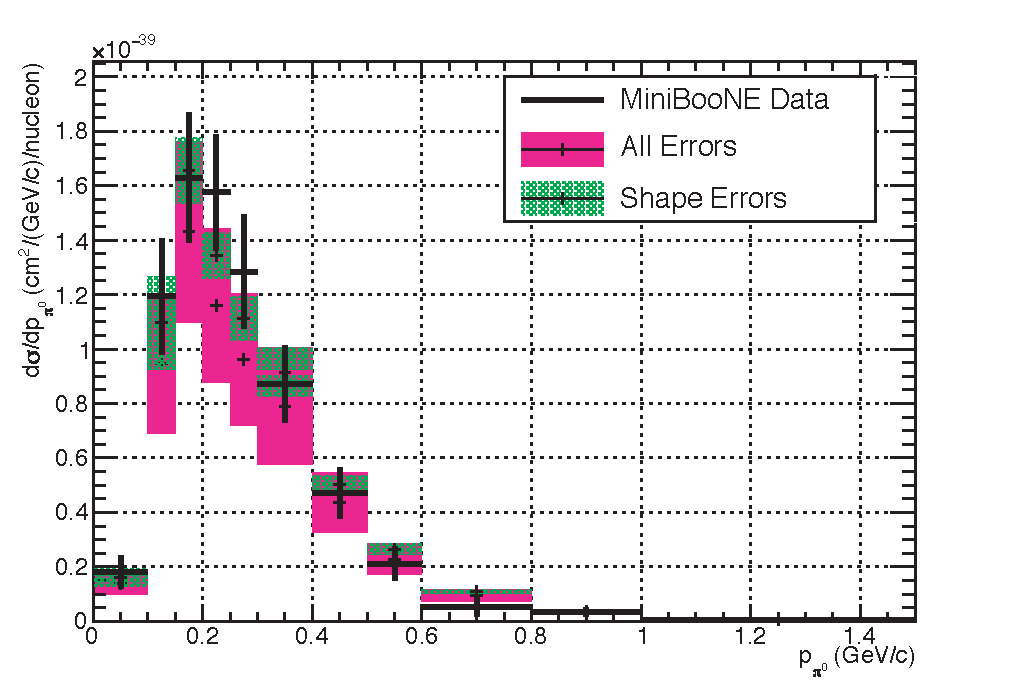
\includegraphics[width=0.8\textwidth]{T2K-TN-254/images/systematics/MB_NC1Pi0_pPi0_nu_curr_good.pdf}\\ %%
  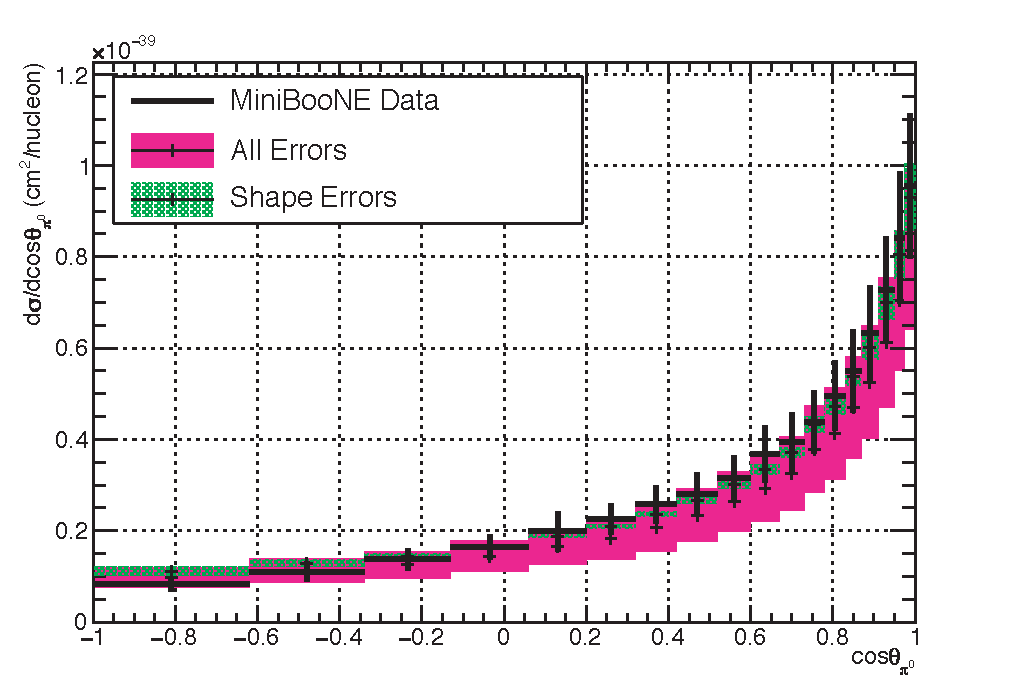
\includegraphics[width=0.8\textwidth]{T2K-TN-254/images/systematics/MB_NC1Pi0_ctPi0_nu_curr_good.pdf} %%
  \caption[MiniBooNE error coverage from current
  parametrisation]{\Gls{MiniBooNE} error coverage from standard
    parametrisation~\cite{TN315} (Table~\ref{tab:reserror}). The black
    line shows the \Gls{MiniBooNE} neutrino mode \Gls{NC}\gls{piz}
    data~\cite{AguilarArevalo:2009ww}, magenta boxes \Gls{NEUT}
    predictions with errors, overlayed green boxes are shape only
    variations from \Gls{NEUT}. \textbf{\textit{Top:}} Pion momentum
    distribution. \textbf{\textit{Bottom:}} Pion angular
    distribution.}
  \label{fig:currenterrors}
\end{figure}

\begin{figure}[ht]
  \center
  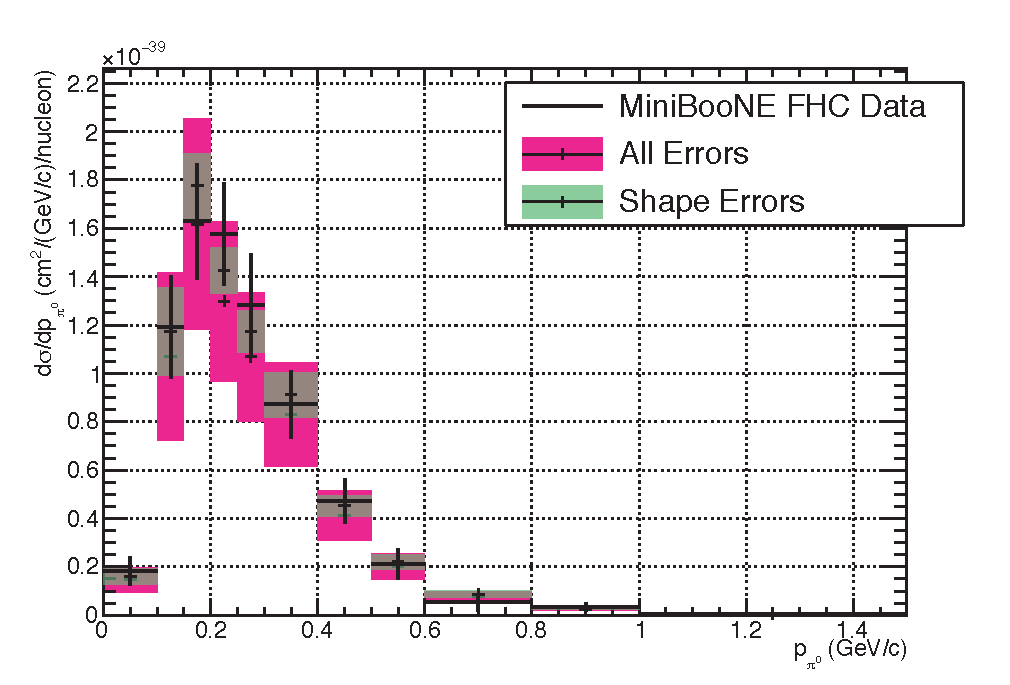
\includegraphics[width=0.8\textwidth]{T2K-TN-254/images/systematics/MB_NC1pi0_1Dppi0_fhc_nu_1WShape_good.pdf}\\ %%
  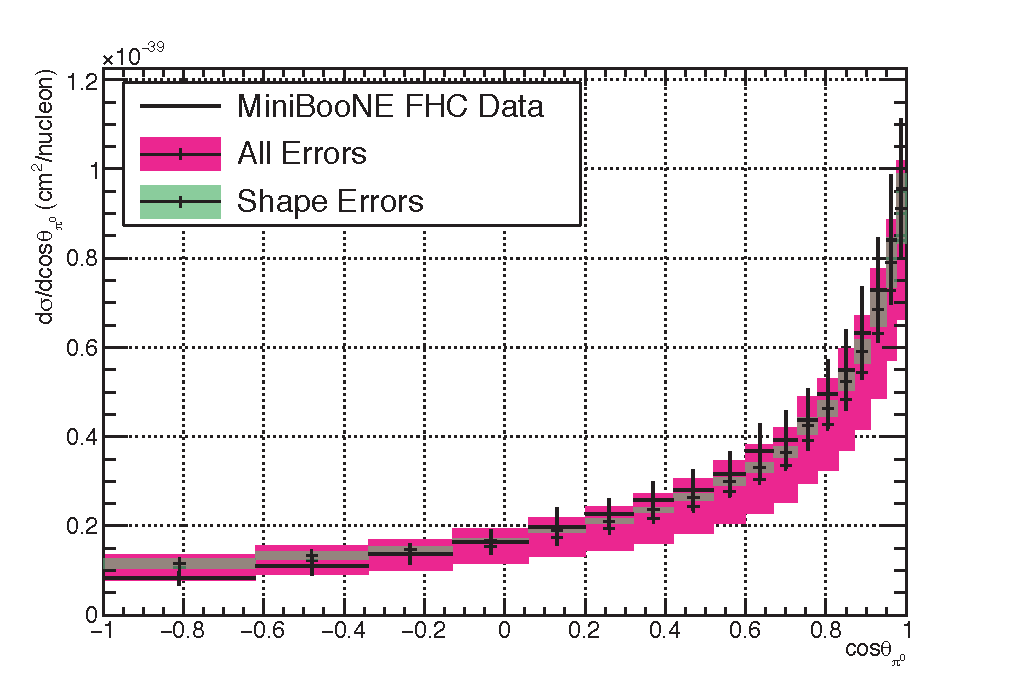
\includegraphics[width=0.8\textwidth]{T2K-TN-254/images/systematics/MB_NC1pi0_1Dcospi0_fhc_nu_1WShape_good.pdf} %%
  \caption[MiniBooNE error coverage using the fitted
  errors]{\Gls{MiniBooNE} error coverage using the fitted errors from
    standard parametrisation~\cite{TN315} (Table~\ref{tab:reserror})
    and $W$-shape error (Table~\ref{tab:fitresult}). The black line
    shows the \Gls{MiniBooNE} neutrino mode \Gls{NC}\gls{piz}
    data~\cite{AguilarArevalo:2009ww}, magenta boxes \Gls{NEUT}
    predictions with errors, overlayed green boxes are shape only
    variations from \Gls{NEUT}. \textbf{\textit{Top:}} Pion momentum
    distribution. \textbf{\textit{Bottom:}} Pion angular
    distribution.}
  \label{fig:miniboonepostfit}
\end{figure}


\begin{figure}[ht]
  \center
  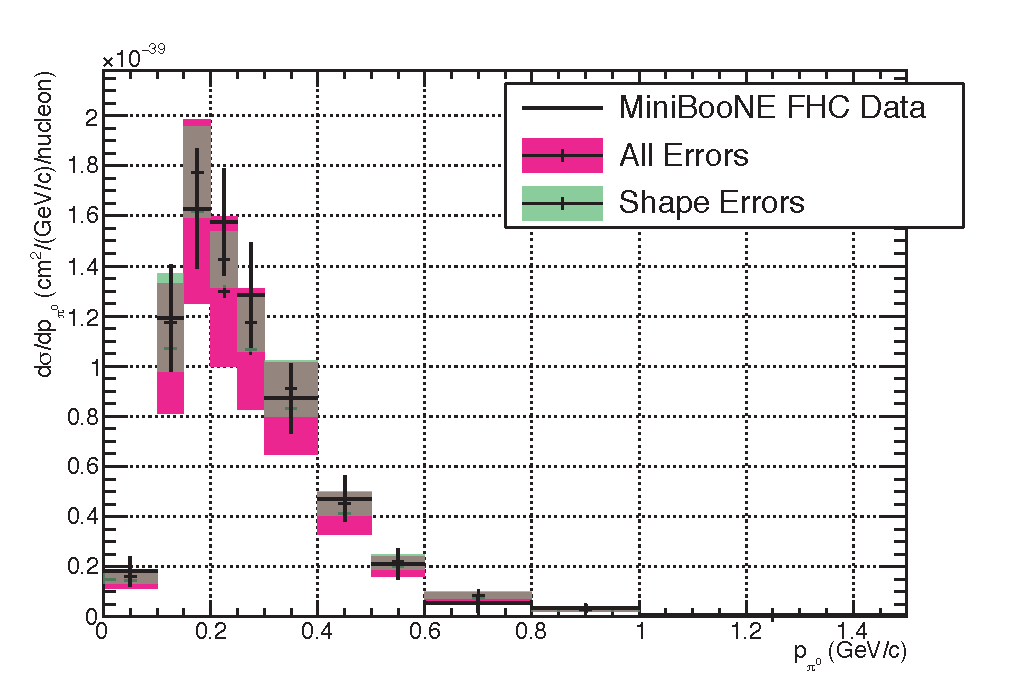
\includegraphics[width=0.8\textwidth]{T2K-TN-254/images/systematics/MB_NC1pi0_1Dppi0_fhc_nu_1WShape_highNCCoh_good.pdf} \\ %%
  \includegraphics[width=0.8\textwidth]{T2K-TN-254/images/systematics/MB_NC1pi0_1Dcospi0_fhc_nu_1WShape_highNCCoh_good.pdf} %%
  \caption[MiniBooNE error coverage using the fitted errors and an
  additional error for NC COH events]{\Gls{MiniBooNE} error coverage
    using the fitted errors from standard parametrisation~\cite{TN315}
    (Table~\ref{tab:reserror}) and from $W$-shape error
    (Table~\ref{tab:fitresult}) with a $100\%$ error on \Gls{NC}
    coherent interaction The black line shows the \Gls{MiniBooNE}
    neutrino mode \Gls{NC}\gls{piz} data~\cite{AguilarArevalo:2009ww},
    magenta boxes \Gls{NEUT} predictions with errors, overlayed green
    boxes are shape only variations from
    \Gls{NEUT}. \textbf{\textit{Top:}} Pion momentum
    distribution. \textbf{\textit{Bottom:}} Pion angular
    distribution.}
  \label{fig:miniboonepostfitcoh}
\end{figure}

\begin{figure}[ht]
  \center
  \includegraphics[width=0.8\textwidth]{T2K-TN-254/images/systematics/MB_NC1Pi0_comp_ppi.pdf} %%
  \includegraphics[width=0.8\textwidth]{T2K-TN-254/images/systematics/MB_NC1Pi0_comp_cospi.pdf} %%
  \caption[MiniBooNE NC$\pi^0$ differential
  distribution]{\Gls{MiniBooNE} \Gls{NC}\gls{piz} differential
    distribution, top: $p_{\pi^{0}}$, bottom:
    $\cos(\theta_{\pi^{0}})$, broken down by \Gls{NEUT} reaction
    modes, the central values and are the same as for
    \ref{fig:miniboonepostfitcoh}.}
  \label{fig:miniboonebreakdown}
\end{figure}

In the case of the \Gls{OOFV} background interactions, they mostly are
from \Gls{RES} interactions, as can be seen in
Tables~\ref{tab:reaction}~and~\ref{tab:target}. The same effects as
described before are also valid so one could wonder if having a carbon
measurement is enough. However, given that there is no
\Gls{NC}\gls{piz} measurement on target other than carbon (and Argon
with \Gls{ArgoNeuT}~\cite{Acciarri:2015ncl}) where the \Gls{piz}
kinematics are available, and the size of the detector error, it was
considered that the differences in uncertainty between carbon and
other nuclear targets should be negligible and thus the uncertainties
described above were applied to the \Gls{OOFV} interactions.

\clearpage

\subsubsection{Relativistic Fermi Gas parameters}
The \Gls{RFG} model is dependent on two fundamental parameters. Both
of them can be determined via electron
scattering~\cite{Alvarez-Ruso:2017oui}.

The first parameter is the Fermi momentum, this quantity is determined
by the width of the elastic peak. The second parameter is the binding
energy, which is determined by the position of the elastic peak. This
quantity corresponds to the energy needed to extract a nucleon from
the Fermi sea.

Unfortunately, even with very accurate electron scattering
measurements, it is hard to find values for these two parameters which
can explain all the electron scattering data~\cite{TN315}, indicating
a deficiency in the model.

The values and uncertainties that are used at \Gls{TK} are listed in
Table~\ref{tab:rfgerror}

\begin{table}[ht]
  \begin{adjustbox}{center}
    \begin{tabular}{cccc}
      \toprule
      Parameter & Value (carbon) & Value (oxygen) & Error \\
      \midrule
      Fermi momentum $p_F$ & $217\text{~MeV}$ & $225\text{~MeV}$ & $31\text{~MeV}$ (flat prior)\\
      Binding energy $E_B$ & $25\text{~MeV}$  & $27\text{~MeV}$  & $9\text{~MeV}$  (flat prior)\\
      \bottomrule
    \end{tabular}
  \end{adjustbox}
  \begin{center}
    \caption[Neutrino RFG errors]{Neutrino \Gls{RFG} errors used
      in the oscillation analysis, reproduced from~\cite{TN315}}
    \label{tab:rfgerror}
  \end{center}
\end{table}

Note that decreasing the $E_B$ parameter ``opens up'' parameter space
(as more events are allowed), and creating a reweighting scheme for
these parameters is not a trivial problem and can lead to significant
bias~\cite{TN315}.

\subsubsection{CCQE Form factor}
Based on bubble chamber data~\cite{ANLCCQE,BNLCCQE,CERNCCQE}, the
\Gls{CCQE} form factor error that is used for the propagation is
$5.8$~\%.

\subsubsection{Multi nucleons}
A $29.5$~\% normalisation uncertainties is assumed for multi-nucleons
events, this comes from analysis from the
\Gls{MINERVA}~\cite{MinervaNuCCQE} and
\Gls{MiniBooNE}~\cite{MiniBooNENuCCQE} experiments.

\subsection{Electron neutrino error}
\label{subsec:electnuerror}
The traditional error for the electron neutrino cross section error is
parametrised as an error on the ratio
$\frac{\sigma_{\text{CC~inc~}\nu_e}}{\sigma_{\text{CC~inc~}\nu_\mu}}$
and similarly for anti-neutrinos. This is admitted to be of the order
of $3\%$, with a $50\%$ correlation for neutrino and anti-neutrino
based on studies in~\cite{Day:2012gb}.

\subsection{Other cross section uncertainty}
\label{subsec:othercrosssection}
Other uncertainties were propagated on the \Gls{DIS} and \Gls{COH}
events. In the case of \Gls{DIS} and \Gls{SIS} events, the scheme is
to reweight the normalisation of the events with an error of the form:
\begin{equation}
  \label{eq:diserror}
  \delta_{\sigma}=\frac{0.4}{E_\nu}
\end{equation}

Which gives an error of $10\%$ at $4$~GeV as was observed
in~\cite{Adamson:2009ju}.

The \Gls{NC} and \Gls{CC} \Gls{COH} events have a normalisation error
of $100\%$ as explained in the previous section.

\subsection{Final State Interactions}
\label{subsec:fsiuncertainty}
Final state interactions denote all the hadron interactions in the
nucleus that happen after the primary neutrino interaction. For
example, if a resonant process happens and creates a pion, this pion
is inside the nucleus and can reinteract in the nucleus. The effect of
the \Gls{FSI} is to generally change the topology of the event (bias
towards lower energy for the pion, absorption of the pion, charge
exchange). However, as discussed earlier, these changes in the shape
have no error (only a normalisation error). For each \Gls{NEUT}
interaction channel of the pion inside the nucleon, an uncertainty is
computed. All the parameters and errors are given in the
Table~\ref{tab:fsiuncertainty}.

\begin{table}[ht]
  \center
  \begin{tabular}{lc}
    \toprule
    Systematic & Relative uncertainty \\
    \midrule
    Pion absorption             & $50\%$  \\
    Low energy charge exchange  & $50\%$  \\
    Low energy quasi elastic    & $50\%$  \\
    Inelastic scattering        & $50\%$  \\
    High energy charge exchange & $30\%$  \\
    High energy quasi elastic   & $30\%$  \\
    \bottomrule
  \end{tabular}
  \caption[FSI parameters and uncertainties]{\Gls{FSI} parameters and
    uncertainties.}
  \label{tab:fsiuncertainty}
\end{table}

For this analysis, the ``16 throws'' method was used. The idea is that
it is sufficient to use sixteen different parameter sets for the
\Gls{FSI} parameters to estimate the systematic error from
\Gls{FSI}. These parameter sets have been detailed in~\cite{TN108} and
are reproduced in Table~\ref{tab:16throws}. The effect of applying
this reweighting is shown in Figure~\ref{fig:fsierror}.

\begin{table}[ht]
  \center
  \begin{tabular}{cccccccc}
    \toprule
    Set & \multicolumn{6}{c}{Parameters} \\ 
        & \multicolumn{2}{c}{Quasi elastic} & Inelastic & Pion       & \multicolumn{2}{c}{Charge exchange}\\
        & LowE  & HighE         & scattering& absorption & LowE &  HighE\\ \midrule
    Nominal  & 1.0  & 1.8   & 1      & 1.1   & 1.0  & 1.8    \\ \midrule
    15 & 0.6  & 1.1   & 1.5    & 0.7   & 0.5  & 2.3    \\
    16 & 0.6  & 1.1   & 1.5    & 0.7   & 1.6  & 2.3    \\
    17 & 0.7  & 1.1   & 1.5    & 1.6   & 0.4  & 2.3    \\
    18 & 0.7  & 1.1   & 1.5    & 1.6   & 1.6  & 2.3    \\
    19 & 1.4  & 1.1   & 1.5    & 0.6   & 0.6  & 2.3    \\
    20 & 1.3  & 1.1   & 1.5    & 0.7   & 1.6  & 2.3    \\
    21 & 1.5  & 1.1   & 1.5    & 1.5   & 0.4  & 2.3    \\
    22 & 1.6  & 1.1   & 1.5    & 1.6   & 1.6  & 2.3    \\ \midrule
    23 & 0.6  & 2.3   & 0.5    & 0.7   & 0.5  & 1.3    \\
    24 & 0.6  & 2.3   & 0.5    & 0.7   & 1.6  & 1.3    \\
    25 & 0.7  & 2.3   & 0.5    & 1.6   & 0.4  & 1.3    \\
    26 & 0.7  & 2.3   & 0.5    & 1.6   & 1.6  & 1.3    \\
    27 & 1.4  & 2.3   & 0.5    & 0.6   & 0.6  & 1.3    \\
    28 & 1.3  & 2.3   & 0.5    & 0.7   & 1.6  & 1.3    \\
    29 & 1.5  & 2.3   & 0.5    & 1.5   & 0.4  & 1.3    \\
    30 & 1.6  & 2.3   & 0.5    & 1.6   & 1.6  & 1.3    \\ \bottomrule
  \end{tabular}
  \caption[The ``16 throws'' parameter sets of the FSI parameters]{The
    ``16 throws'' parameter sets of the \Gls{FSI} parameters.}
  \label{tab:16throws}
\end{table}

\begin{figure}[ht]
  \center
  \includegraphics[width=0.8\textwidth]{images/NCg/FSI.pdf} 
  \caption[Effect of the pion FSI uncertainty on the number of
  selected events]{Effect of the pion \Gls{FSI} uncertainty on the
    number of selected events, using the ``16 throws method''. The
    nominal central value is indicated by the arrow.}
  \label{fig:fsierror}
\end{figure}

Some interactions creating these \Gls{piz} are on heavy elements, such
as the one on the aluminium of the support structure or the lead of
the \Gls{ECal}. Additionally, some interactions on the brass in the
\Gls{PD} can occur.

For the \Gls{FSI}, the \Gls{NEUT} program is used to predict the
pion-nuclear cross section on heavy targets and compared with the
available pion scattering data. A subset of these comparisons is shown
in Figure~\ref{fig:fsiheavy}, which comes from~\cite{FSITalk}, where
all of them are available. Most of the data points lie within the
current error budget, so the errors were not inflated. There is
currently no shape uncertainty for the \Gls{FSI}, and since the
\gls{piz} momentum efficiency is not flat (as can be seen in
Figures~\ref{fig:pizeff1}~and~\ref{fig:pizeff2}), this could lead to
an effect similar to the one described earlier with the Delta mass
parameter. However, \Gls{FSI} shape reweighting will not be done on an
acceptable timescale for the scope of this work; it was therefore
assumed that the normalisation error is sufficient to cover the error.


\begin{figure}[ht]
  \center
  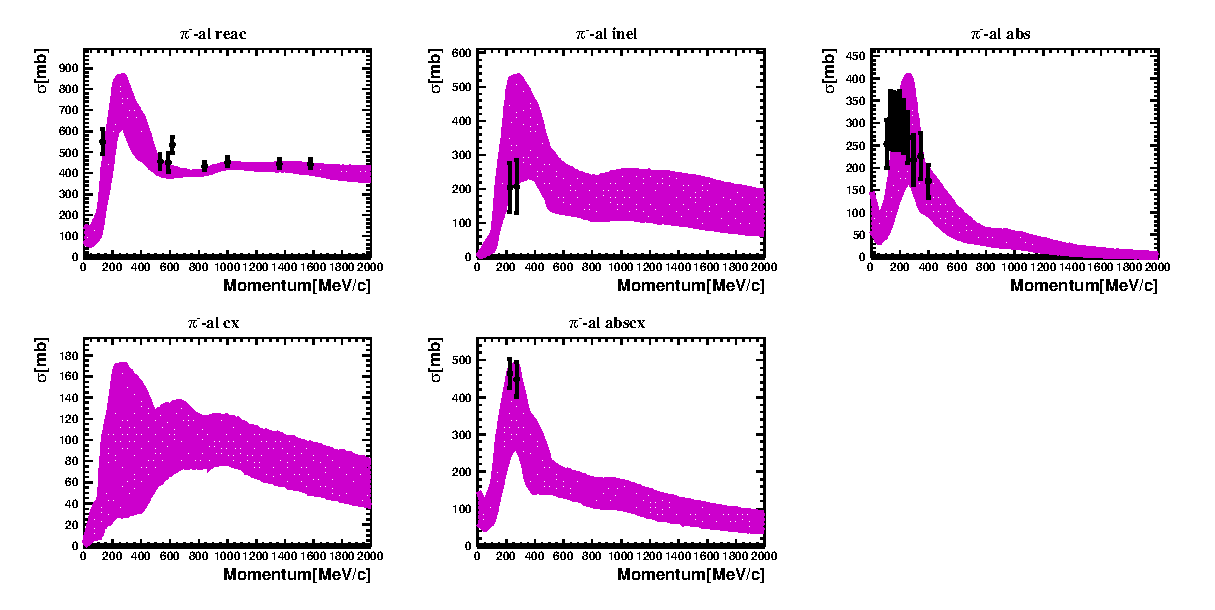
\includegraphics[width=0.9\textwidth]{T2K-TN-254/images/systematics/al_piM_all.eps}
  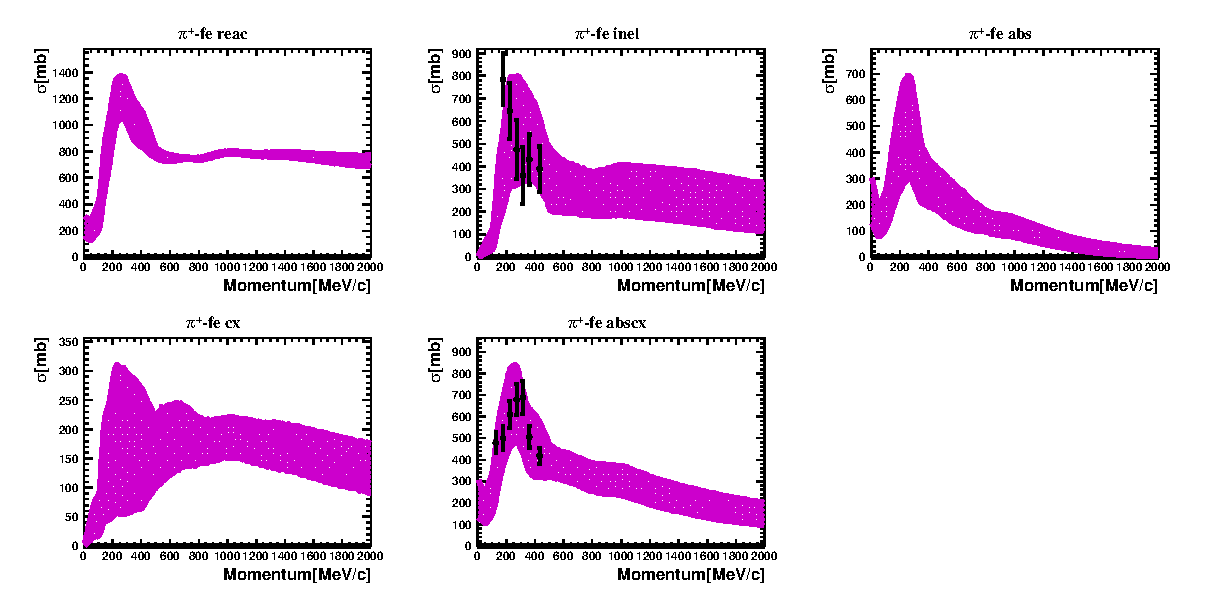
\includegraphics[width=0.9\textwidth]{T2K-TN-254/images/systematics/fe_piP_all.eps} 
  \caption[Comparison of pion scattering data to NEUT prediction and
  uncertainty]{Comparison of pion scattering data to \Gls{NEUT}
    prediction and uncertainty.  \textbf{\textit{Top five:}}
    Negatively charged pion on aluminium.  \textbf{\textit{Bottom
        five:}} Positively charged pion on iron.  From~\cite{FSITalk},
    for references, see in Table~(5.1) of~\cite{TN033}.}
  \label{fig:fsiheavy}
\end{figure}
\clearpage

\subsection{Effects on the selection}

The effects from the nucleon level pion production uncertainties are
shown in Figure~\ref{fig:infvpiproduncertainty}, which shows the
effects on the number of selected events for \Gls{FGD}1 \Gls{FV}
events only. Note that the \Gls{NC} coherent weight distribution shows
a spike at 45 events which corresponds to no coherent events in the
selection. Since the uncertainty is a Gaussian function centred at one
with an error of one; this is expected to happen 16\% of the time.

\begin{figure}[ht]
  \begin{adjustbox}{center}
    \includegraphics[width=0.8\textwidth]{images/NCg/PiProd.pdf} 
  \end{adjustbox}
  \center
  \caption[Effects of the pion resonant cross section uncertainties on
  the number of selected events]{Effects of the pion resonant cross
    section uncertainties on the number of selected events. The
    nominal central value is indicated by the black arrow.}
  \label{fig:infvpiproduncertainty}
\end{figure}

The other \Gls{CCQE} and \gls{nue} cross section errors effects are
shown in Figure~\ref{fig:infvotheruncertainty}.

\begin{figure}[ht]
  \center
  \includegraphics[width=0.8\textwidth]{images/NCg/Other_Jon.pdf} 
  \caption[Effects of the DIS (CC and NC), CCQE, CC coherent and nue
  cross section uncertainty on the number of selected events]{Effects
    of the \Gls{DIS} (\Gls{CC} and \Gls{NC}), \Gls{CCQE}, \Gls{CC}
    coherent and \gls{nue} cross section uncertainty on the number of
    selected events. The nominal central value is indicated by the
    arrow.}
  \label{fig:infvotheruncertainty}
\end{figure}


%%% Local Variables:
%%% mode: latex
%%% TeX-master: Thesis
%%% End:
